\chapter{3D model}
\label{ch:Scene Geometry}
In order to construct the 3D Model of the cabinet the last pieces of information needed are the width of the cabinet panels and the width of one "cell" of the cabinet. To do so, the metric rectification $H_front$ of the front face of the cabinet is needed. That is easily obtained using the calibration matrix as: 
$$
H_{front} = K \cdot \matrixdim{1}{3}{r_1, \hat{r_3} \cdot |r_1|, o_\pi}
$$

Once the image is rectified it is all a matter of taking the right measurements: the width of the cabinet panels is $0.0157$ units long while the width of one "cell" is $0.3167$ units.

The rectified image and the taken references are:
\begin{figure}[H]
\centering
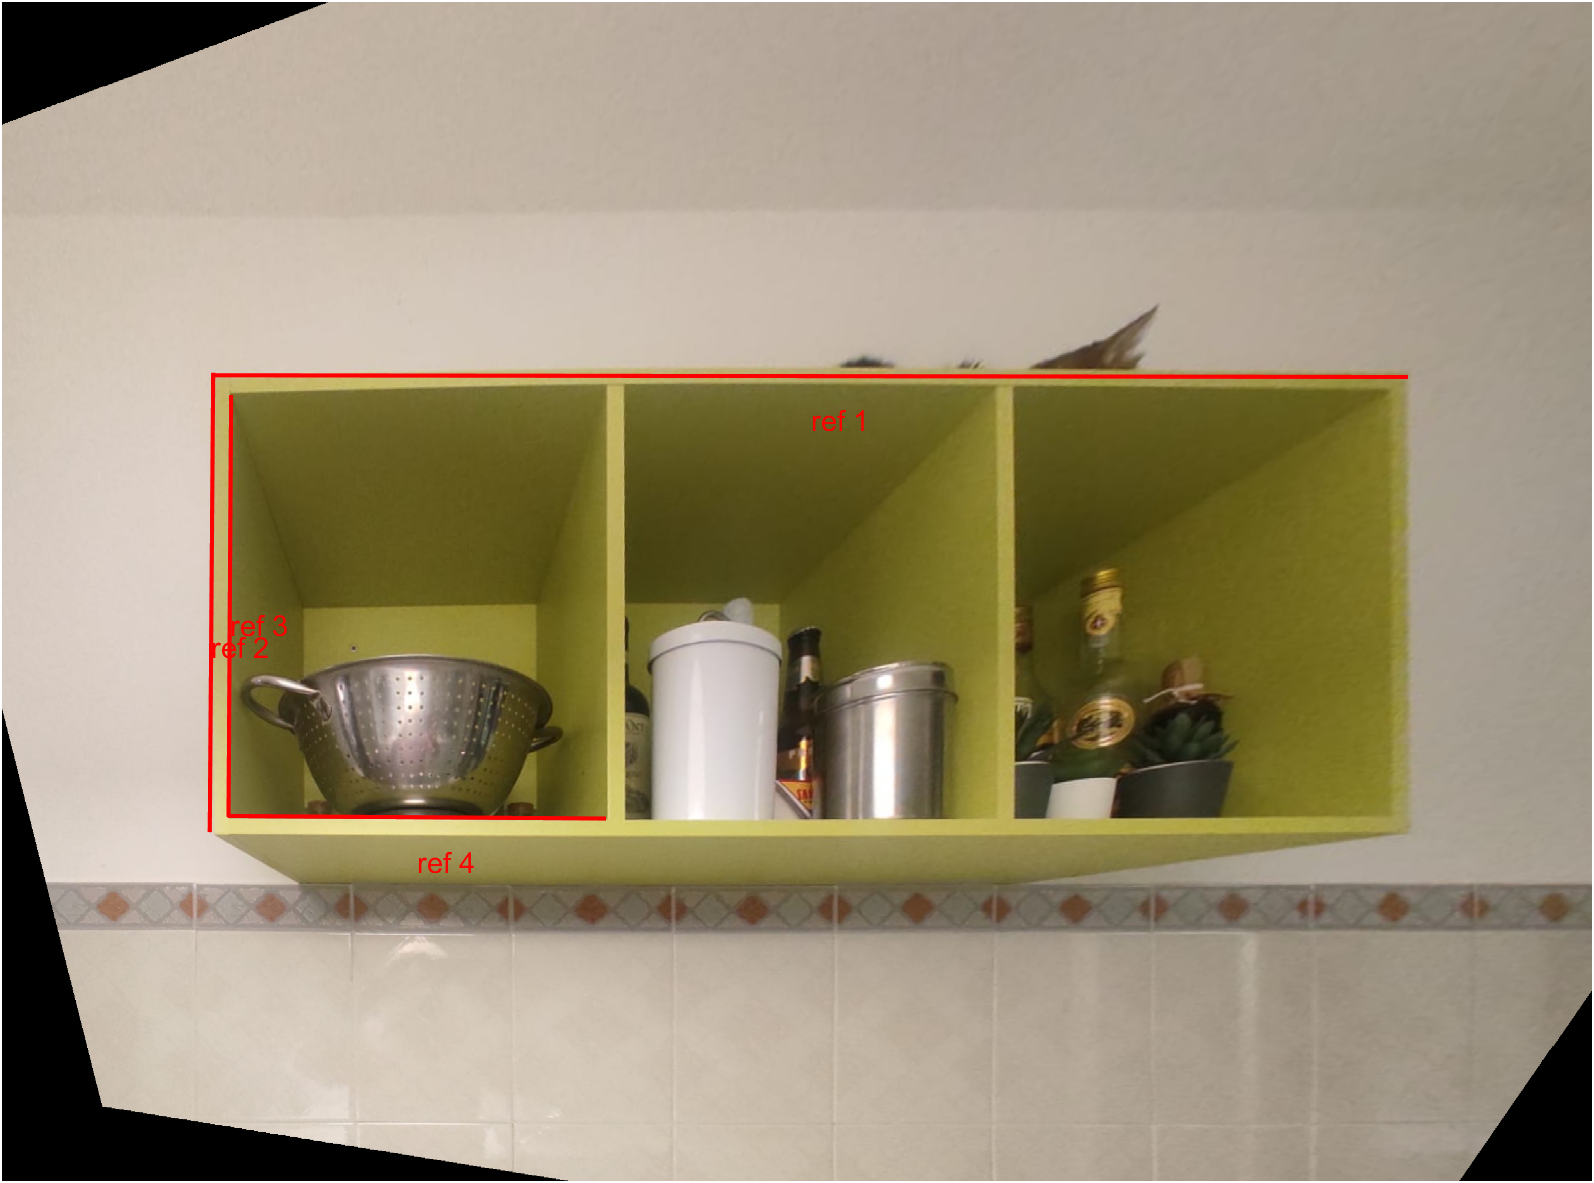
\includegraphics[height=9.5cm, width=\textwidth, keepaspectratio]{Report/Images/2.4-S_coordinated/Vertical Rectification.png}
\caption{\label{fig:Vertical recte}The Metric rectification of the vertical face}
\end{figure}

Using all the information gathered so far a 3D model of the scene can be built:

